% Slug: four-of-diamonds
% Description: ?
% Author: Cisco
% Story: Cisco
% Test Data: Cisco
% Testers: ?
% Editorial: ?
% TempSlug: four-of-diamonds

% Please don't modify or delete TempSlug

\problem{The Rainbow Connection}
Alice, Bob, and Cindy are playing a co-op puzzle game called \textit{The Rainbow Connection}.

In one of the puzzles, there are four columns arranged in a row, each with $n$ nodes labeled $1$ to $n$ from top to bottom.  The spaces between the columns are labeled Zone A, Zone B, and Zone C from left to right.  Here is an illustration of the setup with $n=4$.
\begin{center}
    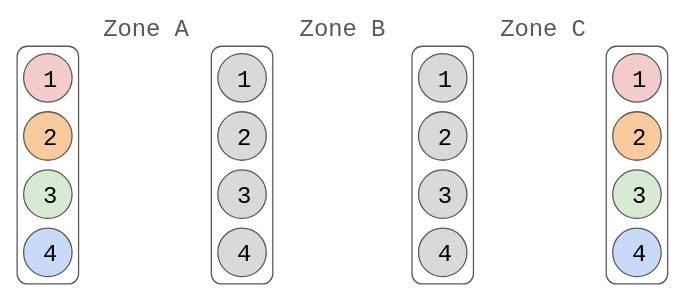
\includegraphics[width=0.575\linewidth]{img/rainbow-b.png}
\end{center}
In this game, you place wires in each of the zones, with each wire connecting a node on the left with some node on the right.

Alice and Cindy got a bit excited and immediately started drawing wires in Zones A and C respectively.  Alice drew $n$ wires, but made it so that there is no node connected to two wires; so did Cindy.  For example, with $n=4$, they might have done the following.
\begin{center}
    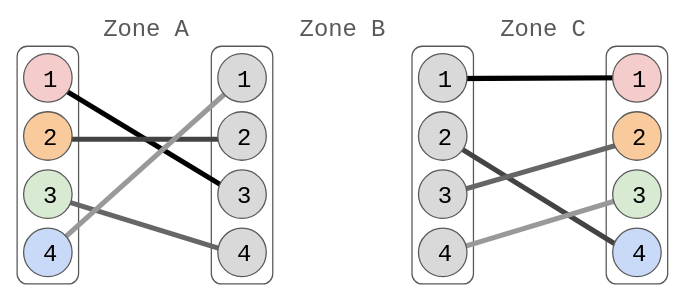
\includegraphics[width=0.575\linewidth]{img/rainbow-1-b.png}
\end{center}
Only after they did this did they read the rules.  They must draw wires such that, for each $i$ from $1$ to $n$: current emitted from the leftmost node $i$ will---if it follows the wires they've drawn---terminate on the rightmost node $i$.

Oops.  Oh well, Bob can still save them, right?  In the example from earlier, the task can still be completed if Bob draws his wires as follows.
\begin{center}
    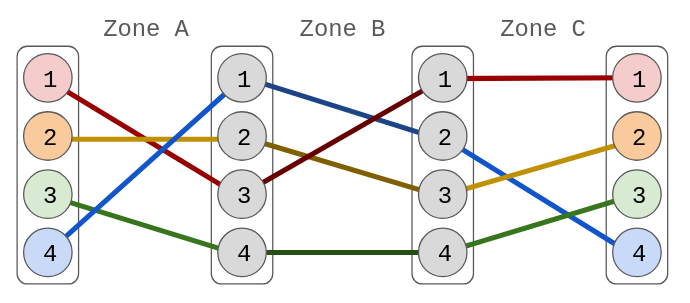
\includegraphics[width=0.575\linewidth]{img/rainbow-2-b.png}
\end{center}

Given the manner in which Alice and Cindy drew their wires, determine how Bob must draw his wires in order for the task to be completed.  It can be shown that the task is always possible.

\subsection*{Input Format}

The first line of input contains a single integer $n$.

The second line of input contains $n$ space-separated integers $a_1, a_2, \dots, a_n$, each a \textit{distinct} integer from $1$ to $n$.  This means that Alice connected node $i$ on her left with node $a_i$ on her right.

The third line of input contains $n$ space-separated integers $c_1, c_2, \dots, c_n$, each a \textit{distinct} integer from $1$ to $n$.  This means that Cindy connected node $i$ on her left with node $c_i$ on her right.

\subsection*{Output Format}

Output $n$ space-separated integers $b_1, b_2, \dots, b_n$, each a \textit{distinct} integer from $1$ to $n$.  This means that Bob will connect node $i$ on his left with node $b_i$ on his right.

If there are multiple possible answers, any will be accepted.

\subsection*{Constraints}

\textit{Your program will only be tested on data that satisfies the following constraints.}

% Set to 10^5 in true bounds
\constraints{
    $2 \leq n \leq 100$ \\
    $a_1, a_2, \dots, a_n$ are distinct integers from $1$ to $n$. \\
    $c_1, c_2, \dots, c_n$ are distinct integers from $1$ to $n$. \\
}

\textit{There is no need to validate in your program that these constraints hold.}

\subsection*{Sample I/O}

\begin{sampleIO}
\begin{verbatim}
4
3 2 4 1
1 4 2 3
\end{verbatim}
&
\begin{verbatim}
2 3 1 4
\end{verbatim}
\end{sampleIO}

\begin{sampleIO}
\begin{verbatim}
7
1 2 3 4 5 6 7
1 2 3 4 5 6 7
\end{verbatim}
&
\begin{verbatim}
1 2 3 4 5 6 7
\end{verbatim}
\end{sampleIO}


% \subsection*{Explanation}
% TODO